\section{Introduction}
\label{sec:introduction}
I like trains
Recently, hybrid rocket engines (HRE) have experienced
a resurgence of popularity as a result of recent technological advances. Hybrid rocket engines combine aspects of both solid and liquid propulsion. From solid motors, they inherit a solid fuel grain which lines the combustion chamber and protects it from hot combusting gasses, and from liquids, they store the oxidizer in a separate fluid tank, allowing for control over the combustion process. Due to their safety, simplicity and throttling capability they have been chosen as the ideal system of in-house propulsion development at Aero Mavs.

\begin{figure}[h]
    \centering
    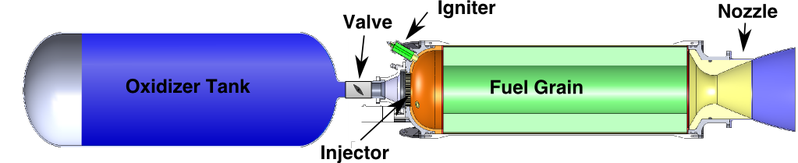
\includegraphics[width=1\linewidth]{Figures/hybridthingi.png}
    \caption{Hybrid Rocket Engine\cite{HybridImage}}
    \label{fig:placeholder1}
\end{figure}

One of the largest issues with traditional hybrid engines is their low regression rate and the secondary issues that this problem creates. Low regression rates are inherent to the way that traditional polymeric fuels combust in the combustion chamber. In a hybrid engine the combustion process takes the form of a long diffusion flame sandwiched in the turbulent boundary layer between the oxidizer plume which originates from the injector on the end of the engine, and the fuel vapor, which is typically generated from the pyrolysis/depolymerization and vaporization of the fuel grain\cite{HumbleHybrid}. Since this interface area and the heat transfer to the fuel grain is limited by the geometry, the reaction rate too is limited, leading to low regression rates compared to solid and liquid propulsion. This characteristic, in turn, introduces several problems in the practical application of hybrid engines. For instance, limited mass flow in the engine limits the total thrust an engine can produce creating scaling issues. While there are various ways to go about mitigating regression rate issues in design, they all have their own downsides, from potentially inducing combustion instability to complicating the manufacturing process or reducing the combustion efficiency. In other words any approach that can inherently increase the regression rates in hybrid fuels would greatly simplify and improve and simplify the practical design of hybrid rocket engines.

\begin{figure}
    \centering
    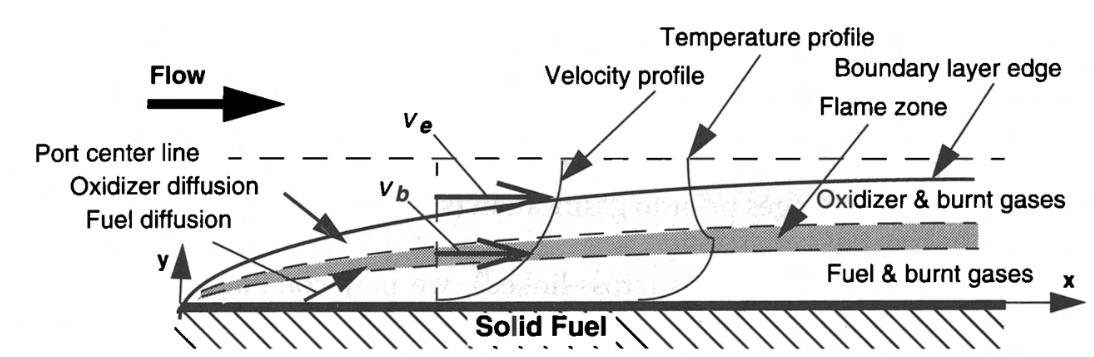
\includegraphics[width=1\linewidth]{Figures/diffusionFlame.png}
    \caption{Diffusion Flame in Hybrid rocket engine\cite{HumbleHybrid}}
    \label{fig:placeholder}
\end{figure}

The way we propose to combat this issue is to improve the reactivity of the fuel under combustion conditions. Due to the inherent safety afforded by separating the fuel and oxidizer before launch, hybrids lend themselves very well to this kind of experimentation and development. 